\chapter{SPOC Hardware and Software Design and Validation}



The SPIN Oscilloscope Shield (SPOC) is used to validate the pins
and signals generated by the \texttt{CUT SPIN}. It
allows up to four selected signals from the 45 available SPIN GPIO pins
to be visualized at the same time on a standard 4-channel oscilloscope.

The main objective is to route selected GPIO signals from the
\texttt{CUT SPIN} to four oscilloscope inputs through
an analog multiplexer network. Each oscilloscope channel independently
displays one selected I/O, which makes it possible to test the complete
board and confirm that the pins behave correctly.

Main requirements:

\begin{itemize}
\item
  cover the 45 available SPIN GPIO pins on each oscilloscope channel
\item
  observe four different GPIO signals at the same time
\item
  route the selected signals to four BNC oscilloscope outputs
\item
  measure real physical signals on the oscilloscope
\item
  verify the complete electrical path from the
  \texttt{CUT SPIN} GPIO to the BNC output
\end{itemize}

This chapter is divided into two main parts. The first part presents the
hardware design and validation of the SPOC oscilloscope shield. The
second part presents the software framework used to automate the PWM
validation workflow.



\newpage
\section{Hardware Design and Validation}

\subsection{GPIO Coverage}\label{gpio-coverage}

The shield is designed to cover the 45 available GPIO pins of the
\texttt{CUT SPIN}. These pins are distributed across the \texttt{PA},
\texttt{PB}, \texttt{PC}, and \texttt{PD} port groups as shown in
Table~\ref{tab:gpio_coverage}.

\begin{table}[H]
\centering
\caption{\texttt{CUT SPIN} GPIO coverage}
\label{tab:gpio_coverage}
\begin{tabular}{|c|l|c|}
\hline
\textbf{Port Group} & \textbf{Pins} & \textbf{Count} \\ \hline
\texttt{PA} & \texttt{PA0--PA10}, \texttt{PA13--PA15} & 14 \\ \hline
\texttt{PB} & \texttt{PB0--PB15} & 16 \\ \hline
\texttt{PC} & \texttt{PC0--PC13} & 14 \\ \hline
\texttt{PD} & \texttt{PD2} & 1 \\ \hline
\multicolumn{2}{|l|}{\textbf{Total GPIO Pins}} & \textbf{45} \\ \hline
\end{tabular}
\end{table}

\subsection{System Architecture}\label{system-architecture}

The validation bench connected to the SPOC shield is built around four elements.

\begin{table}[H]
\centering
\caption{Elements of the SPOC validation bench}
\label{tab:system_elements}
\begin{tabular}{|l|p{10cm}|}
\hline
\textbf{Element} & \textbf{Role} \\ \hline
Computer &
Controls the test sequence, configures the boards, and collects oscilloscope measurements. \\ \hline

CUT SPIN &
Board under test; generates the electrical signals to \newline validate. \\ \hline

MUX SPIN &
Selects which CUT SPIN pins are routed to the shield. \\ \hline

Oscilloscope &
Measures the physical signals available on the BNC \newline outputs. \\ \hline
\end{tabular}
\end{table}
During a test, the computer configures the CUT SPIN, selects the
required route through the mux system, and reads the oscilloscope
measurement. The SPOC shield is the hardware interface between these
elements: it routes the selected GPIO signal to the correct oscilloscope
channel.

\subsection{SPOC Shield Overview}\label{spoc-shield-overview}

Before detailing the internal architecture of the shield, the 3D view
and the real board photograph give an overview of the designed and
manufactured SPOC board. The 3D view shows the placement of the main
connectors and components, while the real photograph presents the
prototype used during the validation phase.

\begin{figure}[H]
\centering
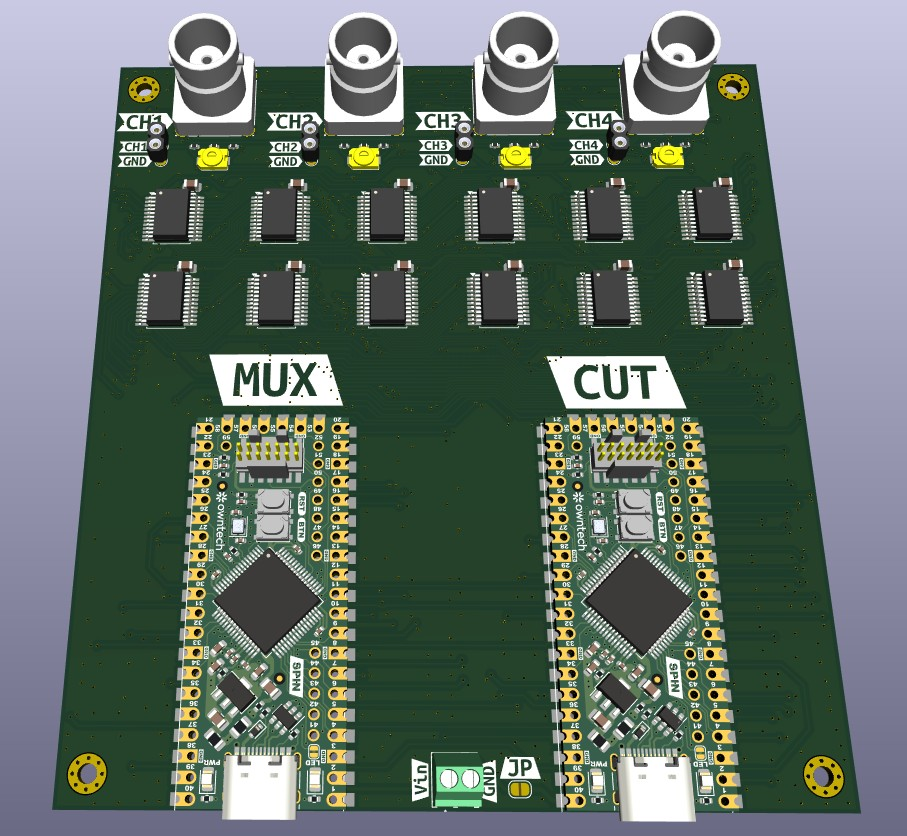
\includegraphics[width=0.9\textwidth]{images/Chapitre 2/spoc_3d.jpg}
\caption{3D view of the SPOC shield}
\label{fig:spoc-3d-view}
\end{figure}


\newpage
\subsection{KiCad Schematic}\label{kicad-schematic}

The shield schematic was designed in KiCad. The schematic shows the
complete board organization: one SPIN board for pin visualization
(\texttt{CUT SPIN}), one SPIN board for mux addressing
(\texttt{MUX SPIN}), and four repeated mux-channel
blocks connected to the oscilloscope outputs.
This top-level view defines how the different functional blocks are
connected before detailing the repeated channel structure.

\begin{figure}[!htbp]
\centering
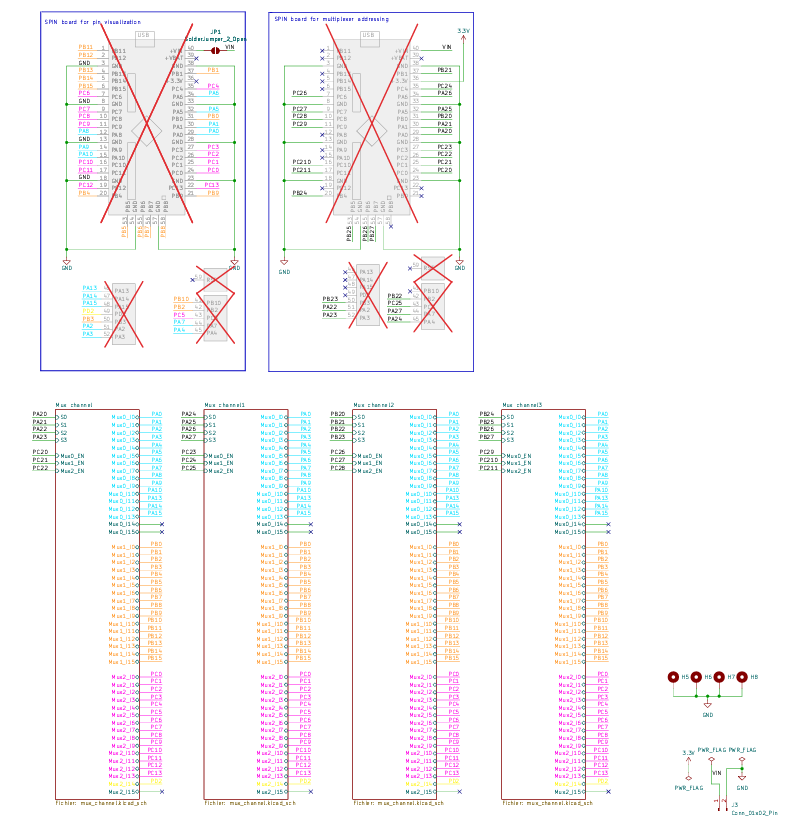
\includegraphics[width=1.05\textwidth]{images/Chapitre 2/IM2.png}
\caption{Top-level KiCad schematic of the SPOC shield}
\end{figure}

\newpage
Each repeated mux-channel block has two groups of inputs:

\begin{itemize}
\item
  on the left side, the mux control inputs come from the
  \texttt{MUX SPIN}
\item
  on the right side, the signals to visualize come from the
  \texttt{CUT SPIN}
\end{itemize}
This separation makes the schematic easier to read: the MUX SPIN
controls the routing logic, while the CUT SPIN provides the signals to
be measured.

\begin{figure}[!htbp]
\centering
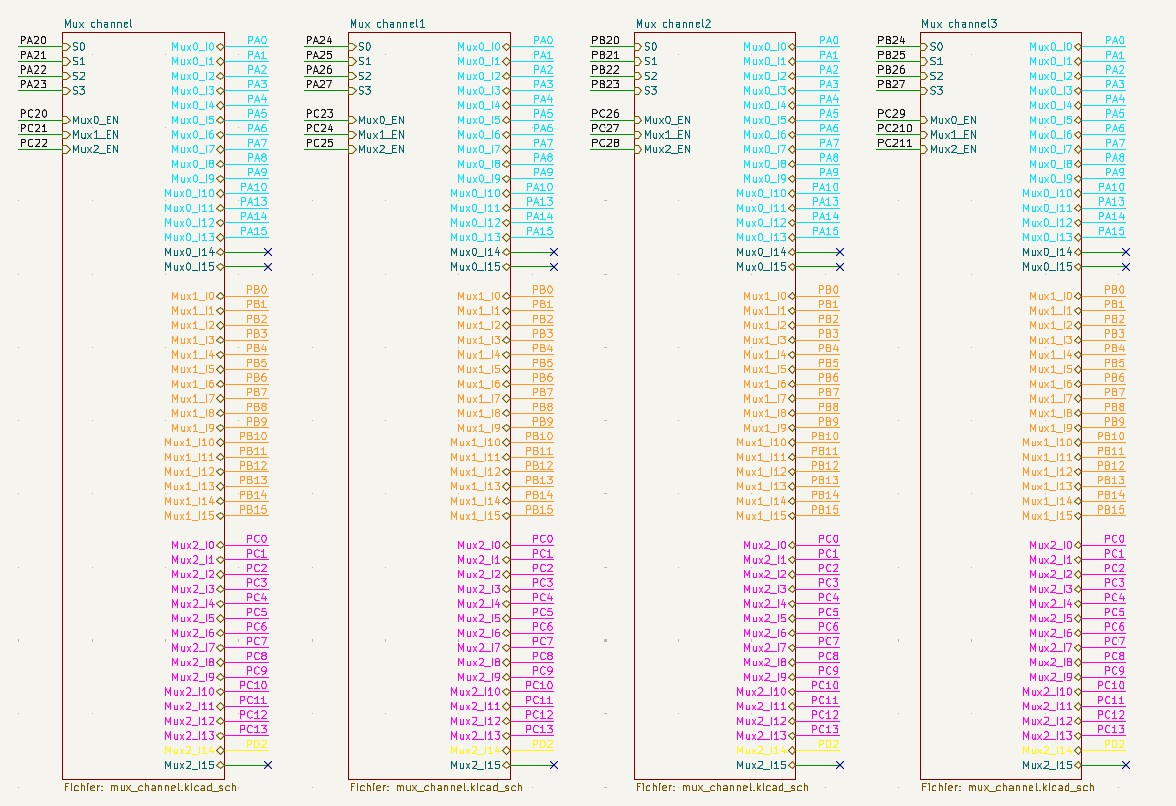
\includegraphics[width=1.00\textwidth]{images/Chapitre 2/IM3.jpg}
\caption{Functional blocks of one mux-channel schematic}
\end{figure}

\newpage
Each mux-channel block contains three \texttt{16:1}
analog multiplexers. The three muxes share the same BNC output path, but
only one mux is enabled at a time. The schematic also includes local
test points, the BNC connector path, decoupling capacitors, and the
output network used for measurement.
This repeated structure is used for all oscilloscope channels, which
keeps the routing principle identical from one channel to another.


\begin{figure}[!htbp]
\centering
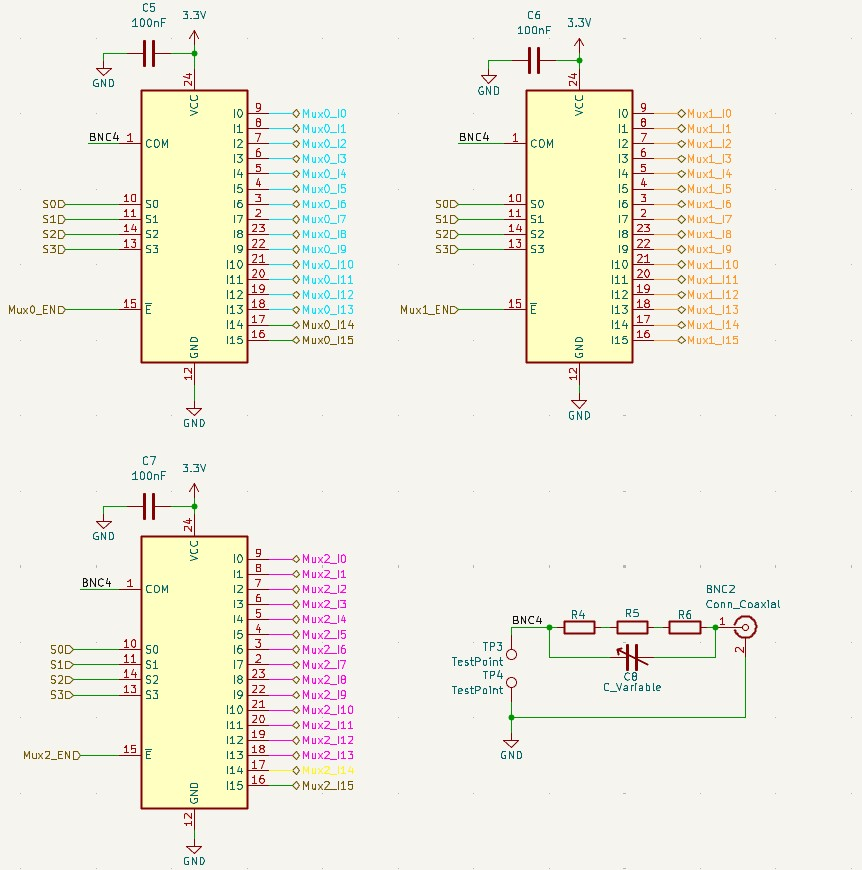
\includegraphics[width=1.00\textwidth]{images/Chapitre 2/IM11.jpg}
\caption{KiCad mux channel schematic}
\end{figure}

\newpage
\subsubsection{BNC Output and Compensation}\label{bnc-output-and-compensation}

Before the BNC connector, the selected signal is available on a local
test point. The BNC output network is inspired by the principle of a
passive \texttt{10x} oscilloscope probe. 

A standard oscilloscope input usually presents a high input impedance,
typically equivalent to \SI{1}{\mega\ohm} to ground. This
high impedance limits the current drawn from the circuit under test, but
the coaxial cable and oscilloscope input also add capacitance. Without
compensation, this capacitance can distort fast waveforms: for example,
a square wave can appear rounded, overshot, or no longer square on the
screen.

To reduce this effect, the SPOC output uses an attenuation and
compensation network. After the local test point, the signal passes
through three \SI{3}{\mega\ohm} resistors in series,
giving a total series resistance of \SI{9}{\mega\ohm}.
Together with the oscilloscope \SI{1}{\mega\ohm} input,
this creates a \texttt{10:1} voltage divider:

\begin{align}
V_{\mathrm{scope}}
  &= V_{\mathrm{signal}}
     \times
     \frac{R_{\mathrm{scope}}}
          {R_{\mathrm{series}} + R_{\mathrm{scope}}} \\
  &= V_{\mathrm{signal}}
     \times
     \frac{\SI{1}{\mega\ohm}}
          {\SI{9}{\mega\ohm} + \SI{1}{\mega\ohm}}  =  \frac{V_{\mathrm{signal}}}{10}
\end{align}

This means the oscilloscope measures one tenth of the real signal
amplitude. For example, a \SI{1}{\volt} signal at the
shield output is measured as about \SI{100}{\milli\volt} at
the oscilloscope input, unless the oscilloscope is configured to display
the corrected \texttt{10x} value. The variable capacitor placed in parallel with the
\SI{9}{\mega\ohm} resistor chain is used for
compensation. Its role is to balance the effect of the cable and input
capacitance so that fast signal edges are preserved more correctly. If
the compensation is not adjusted correctly, the output network can
behave like a low-pass or high-pass filter and distort the measured
waveform. The compensation can be checked with a calibrated square-wave
signal and adjusted until the displayed waveform remains square.

\begin{figure}[!htbp]
\centering
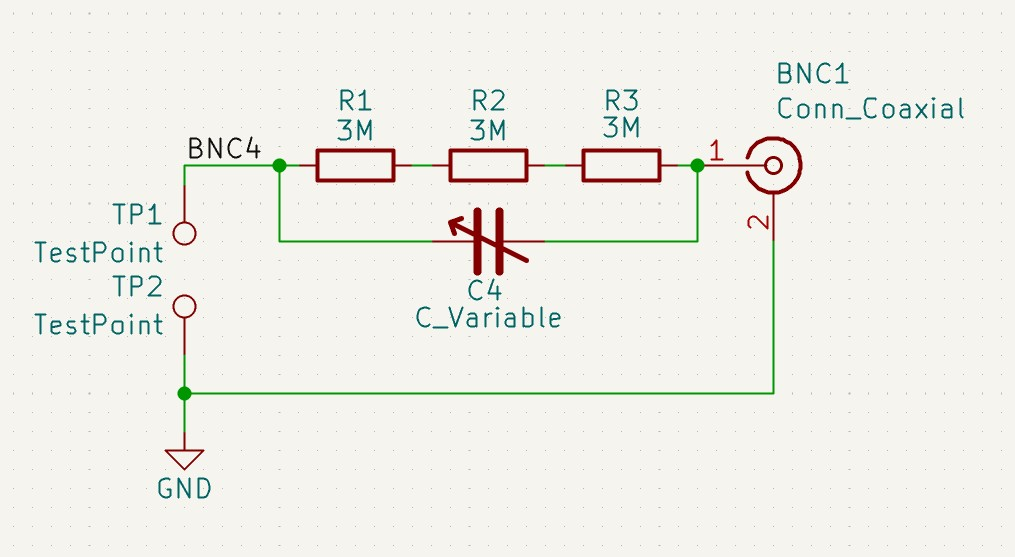
\includegraphics[width=0.45\textwidth]{images/Chapitre 2/IM4.jpg}
\caption{BNC output compensation network}
\end{figure}


\subsection{Multiplexer Architecture}\label{multiplexer-architecture}

The SPOC shield uses \texttt{CD74HC4067SM96} \texttt{16:1} analog
multiplexers. Each oscilloscope channel consists of three multiplexers
sharing a common output path, a local test point, and a BNC connector.
Since these devices are analog multiplexers, they can route both digital
logic levels and analog waveforms from the selected SPIN GPIO to the
oscilloscope. The SPOC shield uses CD74HC4067 analog
multiplexers~\cite{ti_cd74hc4067}.


The complete board uses:

\begin{table}[H]
\centering
\caption{Hardware resources}
\label{tab:hardware_resources}
\begin{tabular}{|l|l|}
\hline
\textbf{Hardware item} & \textbf{Quantity} \\ \hline
\texttt{16:1} analog muxes & 12 total, 3 per channel \\ \hline
Mux address lines & 16 \texttt{MUX SPIN} GPIO controls, \texttt{S0--S3} for each channel \\ \hline
Mux enable lines & 12 \texttt{MUX SPIN} GPIO controls, one enable per mux \\ \hline
BNC outputs & 4, one per oscilloscope channel \\ \hline
\end{tabular}
\end{table}

\subsubsection{Channel Principle}\label{channel-principle}

\texttt{CH1} is used as the reference channel because
\texttt{CH2}, \texttt{CH3}, and \texttt{CH4} repeat the same structure.
The selected signal passes through one enabled mux group, then reaches
the local test point and the corresponding BNC output.

The selection logic is:

\begin{itemize}
\item \texttt{S0..S3} select the input address inside the active mux.
\item \texttt{EN\_MUX1}, \texttt{EN\_MUX2}, or \texttt{EN\_MUX3} chooses which mux group is connected to the channel output.
\item Only one mux enable line should be driven low at a time.
\item The selected signal appears on the local test point and on the channel BNC output.
\end{itemize}








The \texttt{CD74HC4067} enable input is active low.
This means a mux is enabled when its \texttt{EN\_MUXx} signal is driven low, and disabled when the enable signal is high. For each channel, the \texttt{MUX SPIN} must therefore keep only the selected mux enable line low and keep the other mux enable lines high.



Each channel uses the same input-family organization:

\begin{table}[H]
\centering
\caption{\texttt{CUT SPIN} GPIO input-family organization}
\label{tab:mux_input_family_organization}
\begin{tabular}{|c|l|c|}
\hline
\textbf{Mux} & \textbf{\texttt{CUT SPIN} GPIO family} & \textbf{Address range} \\ \hline
\texttt{MUX1} & \texttt{PA0--PA10}, \texttt{PA13--PA15} & \texttt{0--13} \\ \hline
\texttt{MUX2} & \texttt{PB0--PB15} & \texttt{0--15} \\ \hline
\texttt{MUX3} & \texttt{PC0--PC13}, \texttt{PD2} & \texttt{0--14} \\ \hline
\end{tabular}
\end{table}

Example: to display \texttt{PB6} from the \texttt{CUT SPIN} on \texttt{CH1}, the signal belongs to the \texttt{MUX2} group. \texttt{MUX2} is enabled and the selected address is \texttt{6}, or \texttt{0110} on \texttt{S0..S3}. Because the mux enable input is active low, the enable states are \texttt{EN\_MUX1 = 1}, \texttt{EN\_MUX2 = 0}, and \texttt{EN\_MUX3 = 1}. The same logic is repeated independently for \texttt{CH1}, \texttt{CH2}, \texttt{CH3}, and \texttt{CH4}.


\subsubsection{Channel Areas}\label{channel-areas}

The four oscilloscope channels use the same mux structure. The input
families stay identical for every channel: \texttt{MUX1} routes the
\texttt{PA} family, \texttt{MUX2} routes the \texttt{PB} family, and
\texttt{MUX3} routes the \texttt{PC}/\texttt{PD2} family. What changes
from one channel to another is the physical PCB area and the set of
\texttt{MUX SPIN} control pins assigned to that channel.

\begin{figure}[!htbp]
\centering
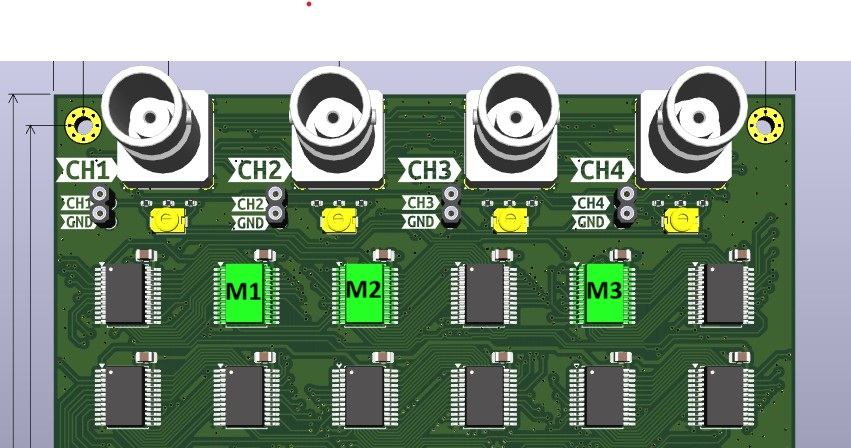
\includegraphics[width=0.70\textwidth]{images/Chapitre 2/MUX_CH1.jpg}
\caption{CH1 mux area}
\end{figure}

\begin{figure}[H]
\centering
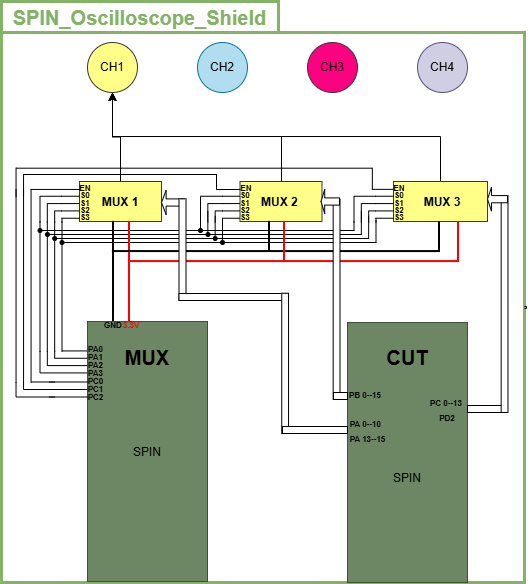
\includegraphics[width=0.65\textwidth]{images/Chapitre 2/SPIN_Oscilloscope_Shield-CablageCH1.png}
\caption{SPIN Oscilloscope Shield CH1 cabling}
\end{figure}


The \texttt{CH1} figures are used as the detailed example. The same
principle is repeated for \texttt{CH2}, \texttt{CH3}, and \texttt{CH4}:
each channel has its own three-mux block, its own control pins, one local
test point, and one BNC output. Only the PCB position and the assigned
\texttt{MUX SPIN} pins change from one channel to another.

\begin{figure}[!htbp]
\centering
\begin{subfigure}{0.32\textwidth}
\centering
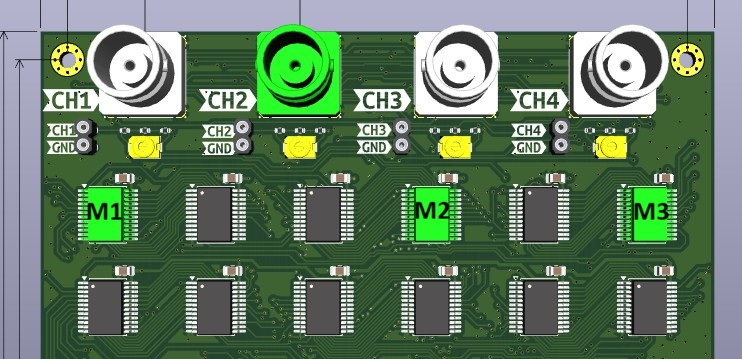
\includegraphics[width=\textwidth]{images/Chapitre 2/MUX_CH2.jpg}
\caption{\texttt{CH2}}
\end{subfigure}
\hfill
\begin{subfigure}{0.32\textwidth}
\centering
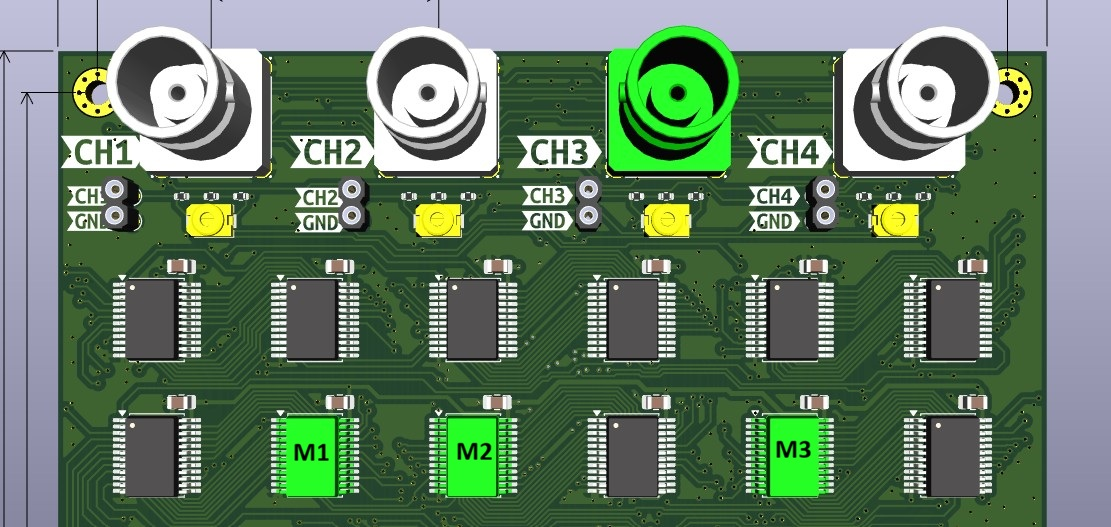
\includegraphics[width=\textwidth]{images/Chapitre 2/MUX_CH3.jpg}
\caption{\texttt{CH3}}
\end{subfigure}
\hfill
\begin{subfigure}{0.32\textwidth}
\centering
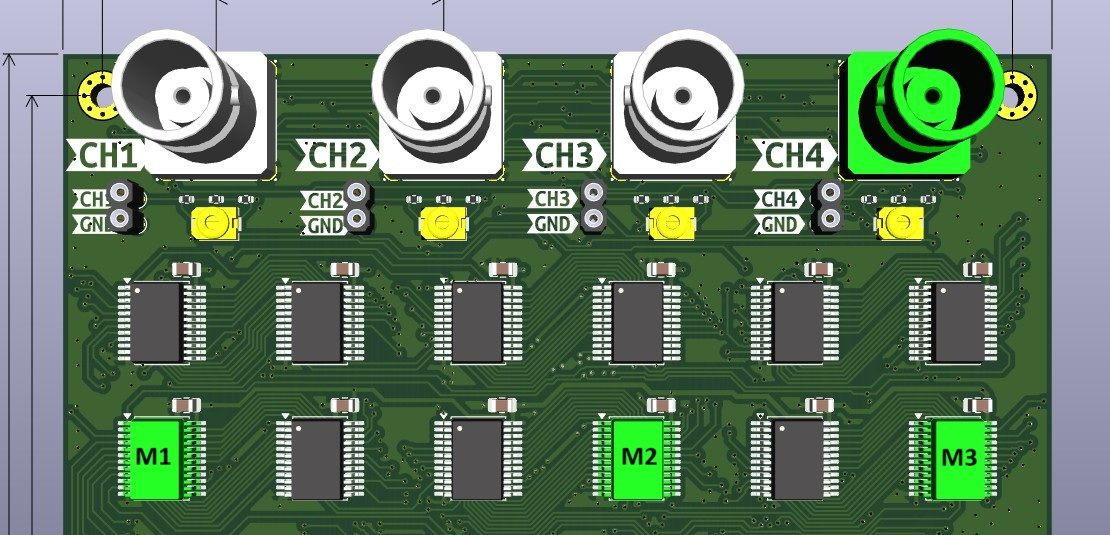
\includegraphics[width=\textwidth]{images/Chapitre 2/MUX_CH4.jpg}
\caption{\texttt{CH4}}
\end{subfigure}
\caption{Mux areas for the remaining oscilloscope channels}
\end{figure}

\FloatBarrier
\newpage
\subsubsection{Control Pin Mapping}\label{control-pin-mapping}

The following tables summarize the \texttt{MUX SPIN} GPIO pins used to
control the address and enable signals, and the \texttt{CUT SPIN} GPIO
pins connected to each mux input address.

\begingroup
\small
\setlength{\tabcolsep}{4pt}
\renewcommand{\arraystretch}{1.3}
\setlength{\abovecaptionskip}{5pt}
\setlength{\belowcaptionskip}{5pt}

\begin{center}
\captionof{table}{MUX SPIN control pin mapping}
\label{tab:control_pin_mapping}
\resizebox{\textwidth}{!}{%
\begin{tabular}{|c|c|c|c|c|c|c|c|}
\hline
\textbf{Channel} & \textbf{S0} & \textbf{S1} & \textbf{S2} & \textbf{S3} &
\textbf{EN\_MUX1} & \textbf{EN\_MUX2} & \textbf{EN\_MUX3} \\ \hline
\texttt{CH1} & \texttt{PA0} & \texttt{PA1} & \texttt{PA2} & \texttt{PA3} & \texttt{PC0} & \texttt{PC1} & \texttt{PC2} \\ \hline
\texttt{CH2} & \texttt{PA4} & \texttt{PA5} & \texttt{PA6} & \texttt{PA7} & \texttt{PC3} & \texttt{PC4} & \texttt{PC5} \\ \hline
\texttt{CH3} & \texttt{PB0} & \texttt{PB1} & \texttt{PB2} & \texttt{PB3} & \texttt{PC6} & \texttt{PC7} & \texttt{PC8} \\ \hline
\texttt{CH4} & \texttt{PB4} & \texttt{PB5} & \texttt{PB6} & \texttt{PB7} & \texttt{PC9} & \texttt{PC10} & \texttt{PC11} \\ \hline
\end{tabular}
}
\end{center}


\begin{center}
\captionof{table}{\texttt{CUT SPIN} GPIO to multiplexer input mapping}
\label{tab:gpio_mux_mapping}
\begin{tabular}{|c|p{3.9cm}|p{3.9cm}|p{3.9cm}|}
\hline
\textbf{Address} &
\textbf{MUX1 input from CUT SPIN} &
\textbf{MUX2 input from CUT SPIN} &
\textbf{MUX3 input from CUT SPIN} \\ \hline
0  & \texttt{I0 / PA0}   & \texttt{I0 / PB0}   & \texttt{I0 / PC0} \\ \hline
1  & \texttt{I1 / PA1}   & \texttt{I1 / PB1}   & \texttt{I1 / PC1} \\ \hline
2  & \texttt{I2 / PA2}   & \texttt{I2 / PB2}   & \texttt{I2 / PC2} \\ \hline
3  & \texttt{I3 / PA3}   & \texttt{I3 / PB3}   & \texttt{I3 / PC3} \\ \hline
4  & \texttt{I4 / PA4}   & \texttt{I4 / PB4}   & \texttt{I4 / PC4} \\ \hline
5  & \texttt{I5 / PA5}   & \texttt{I5 / PB5}   & \texttt{I5 / PC5} \\ \hline
6  & \texttt{I6 / PA6}   & \texttt{I6 / PB6}   & \texttt{I6 / PC6} \\ \hline
7  & \texttt{I7 / PA7}   & \texttt{I7 / PB7}   & \texttt{I7 / PC7} \\ \hline
8  & \texttt{I8 / PA8}   & \texttt{I8 / PB8}   & \texttt{I8 / PC8} \\ \hline
9  & \texttt{I9 / PA9}   & \texttt{I9 / PB9}   & \texttt{I9 / PC9} \\ \hline
10 & \texttt{I10 / PA10} & \texttt{I10 / PB10} & \texttt{I10 / PC10} \\ \hline
11 & \texttt{I11 / PA13} & \texttt{I11 / PB11} & \texttt{I11 / PC11} \\ \hline
12 & \texttt{I12 / PA14} & \texttt{I12 / PB12} & \texttt{I12 / PC12} \\ \hline
13 & \texttt{I13 / PA15} & \texttt{I13 / PB13} & \texttt{I13 / PC13} \\ \hline
14 & --                  & \texttt{I14 / PB14} & \texttt{I14 / PD2} \\ \hline
15 & --                  & \texttt{I15 / PB15} & -- \\ \hline
\end{tabular}
\end{center}

\endgroup

\clearpage

\subsection{PCB Layout and Stackup}\label{pcb-layout-and-stackup}

The SPOC shield PCB was routed as a \texttt{4-layer} board. The external layers are used for signal routing, 
while the internal layers are used as \texttt{GND} reference planes for current return paths.

\begin{table}[H]
\centering
\caption{PCB layer stack-up}
\label{tab:pcb_layers}
\begin{tabular}{|c|l|p{7cm}|}
\hline
\textbf{Layer} & \textbf{Main role} & \textbf{Routing direction / use} \\ \hline
\texttt{F.Cu} & Signal routing & Mostly horizontal signal traces, shown in red. \\ \hline
\texttt{In1.Cu} & Ground plane & Internal \texttt{GND} layer for return current. \\ \hline
\texttt{In2.Cu} & Ground plane & Internal \texttt{GND} layer for return current. \\ \hline
\texttt{B.Cu} & Signal routing & Mostly vertical signal traces, shown in blue. \\ \hline
\end{tabular}
\end{table}

The internal \texttt{GND} planes provide a close reference plane for the signal traces. 
This improves the return-current path, reduces the loop area, and helps keep the oscilloscope signals cleaner during switching.

\vspace{1 cm}
The routing widths are:

\begin{table}[H]
\centering
\caption{PCB track widths}
\label{tab:track_widths}
\begin{tabular}{|l|c|}
\hline
\textbf{Net type} & \textbf{Track width} \\ \hline
Signal traces & 0.2 mm \\ \hline
Power supply traces & 0.5 mm \\ \hline
\end{tabular}
\end{table}

To achieve a more compact PCB layout, 
signal traces on the \texttt{F.Cu} layer were routed mainly in the horizontal direction, 
whereas traces on the \texttt{B.Cu} layer were routed mainly in the vertical direction. 
This routing strategy reduces trace crossings and optimizes the use of the available board area.



\subsection{Power Supply Jumper}\label{power-supply-jumper}

A \texttt{VIN} jumper was added to control the power
link between the two SPIN boards. The jumper avoids unintentionally
connecting the two \texttt{VIN} lines through the USB
cable. When the jumper is soldered, both SPIN boards can be powered from
a single USB cable.

\begin{figure}[H]
\centering
\begin{minipage}{0.48\textwidth}
    \centering
    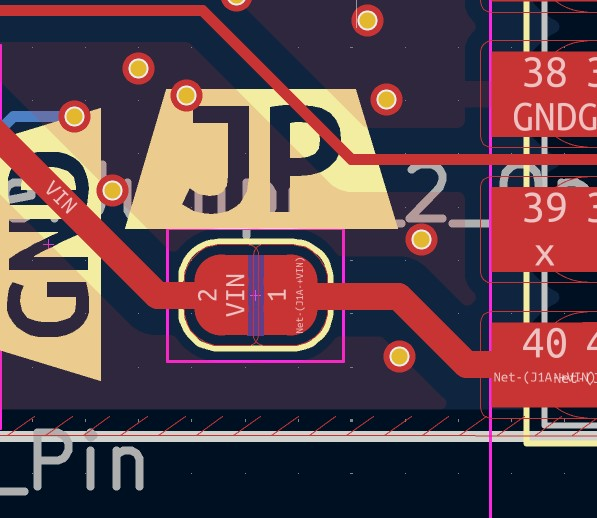
\includegraphics[width=0.9\linewidth]{images/Chapitre 2/IM9.jpg}
    \caption{VIN jumper schematic}
    \label{fig:vin_schematic}
\end{minipage}
\hfill
\begin{minipage}{0.45\textwidth}
    \centering
    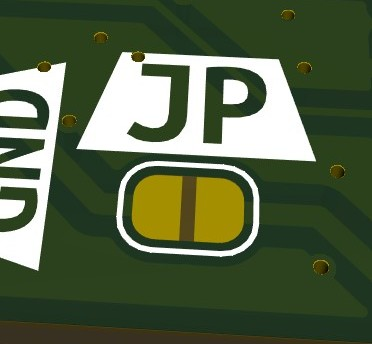
\includegraphics[width=0.9\linewidth]{images/Chapitre 2/IM10.jpg}
    \caption{VIN jumper location on the PCB}
    \label{fig:vin_location}
\end{minipage}
\end{figure}

\subsection{Hardware Bring-Up and Validation}\label{hardware-bring-up-and-validation}

This section groups the physical board checks performed after assembly:
power verification, routing validation, and output calibration
observations.

\subsubsection{Power Checks}\label{power-checks}

Before functional testing, the board was checked for shorts and correct
supply rails. The important hardware checks passed:
\texttt{VIN}, \texttt{3.3V},
\texttt{GND}, BNC shield ground, and mux supply
continuity.

\begin{table}[H]
\centering
\caption{Measured supply voltages}
\label{tab:supply_voltage_measurements}
\begin{tabular}{|c|c|c|}
\hline
\textbf{Rail} & \textbf{Measured value} & \textbf{Result} \\ \hline
\texttt{VIN} & \SI{4.743}{\volt} & PASS \\ \hline
\texttt{3.3V} & \SI{3.286}{\volt} & PASS \\ \hline
\end{tabular}
\end{table}

No abnormal heating was observed during first power-up.

\subsubsection{Hardware Validation}\label{hardware-validation}

The selected signal was checked from the
\texttt{CUT SPIN} GPIO through the mux network to the
test point and BNC output. The hardware validation confirmed:

\begin{itemize}
\item
  the selected signal appears on the expected channel
\item
  mux addressing works
\item
  mux enable behavior works
\item
  the local test point and BNC output match
\item
  no unexpected coupling was observed between channels
\end{itemize}

An early issue was found on some \texttt{MUX1 / CH1}
routes. After resoldering the interior
\texttt{CUT SPIN} pins, the failing routes worked
correctly.

After correction, all \texttt{180} tested routes passed
successfully, with \texttt{0} failed routes.

\subsubsection{Offset and Calibration Observation}\label{offset-and-calibration-observation}

After observing an output offset on the \texttt{BNC}
outputs during measurement, and after identifying the same behavior in
simulation, a calibration stage was added after the functional hardware
verification. The purpose of this step is to better characterize the
offset behavior and apply the required correction for improved
measurement accuracy.

Offset without output:

\begin{figure}[!htbp]
\centering
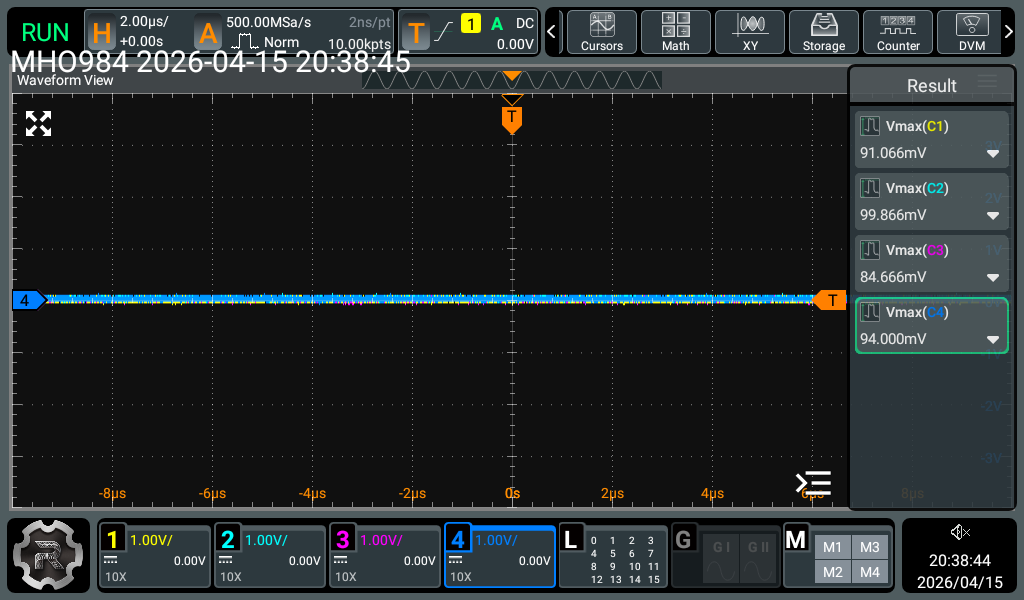
\includegraphics[width=1\textwidth]{images/Chapitre 2/offset0.png}
\caption{BNC output offset measured without input signal}
\end{figure}

The DC calibration setup compares three points at the same time:

\begin{itemize}
\item
  \texttt{VCUT}: signal directly from the
  \texttt{CUT SPIN}, measured on oscilloscope
  \texttt{CH2}
\item
  \texttt{VTEST}: signal at the local test point,
  measured on oscilloscope \texttt{CH3}
\item
  \texttt{VBNC}: signal at the
  \texttt{BNC} output, measured on oscilloscope
  \texttt{CH1}
\end{itemize}

This setup makes it possible to compare the generated source signal, the
local routed signal on the shield, and the final
\texttt{BNC} output.

\begin{figure}[!htbp]
\centering

\begin{subfigure}{0.40\textwidth}
    \centering
    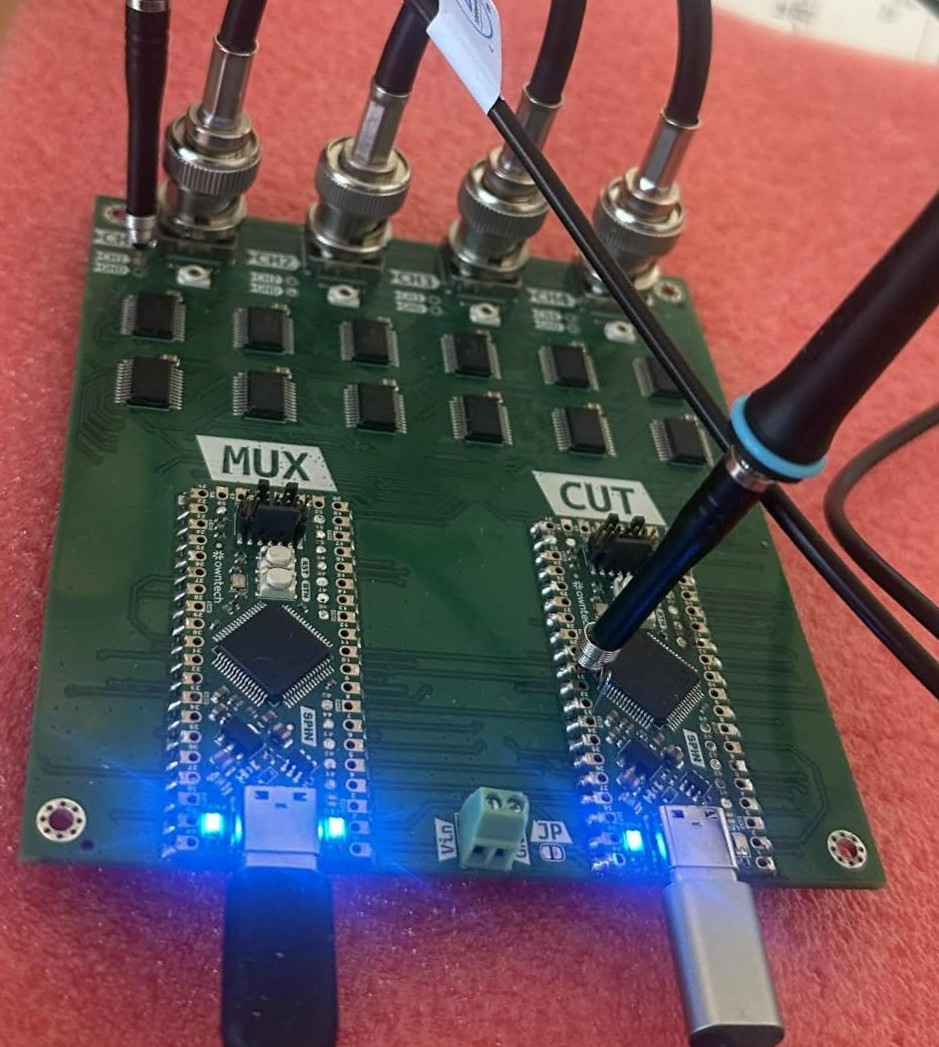
\includegraphics[width=\linewidth]{images/Chapitre 2/ab316f4e-eec0-4d3a-8e9a-5ac785216647.jpeg}
    \caption{Bench calibration setup}
\end{subfigure}
\hfill
\begin{subfigure}{0.55\textwidth}
    \centering
    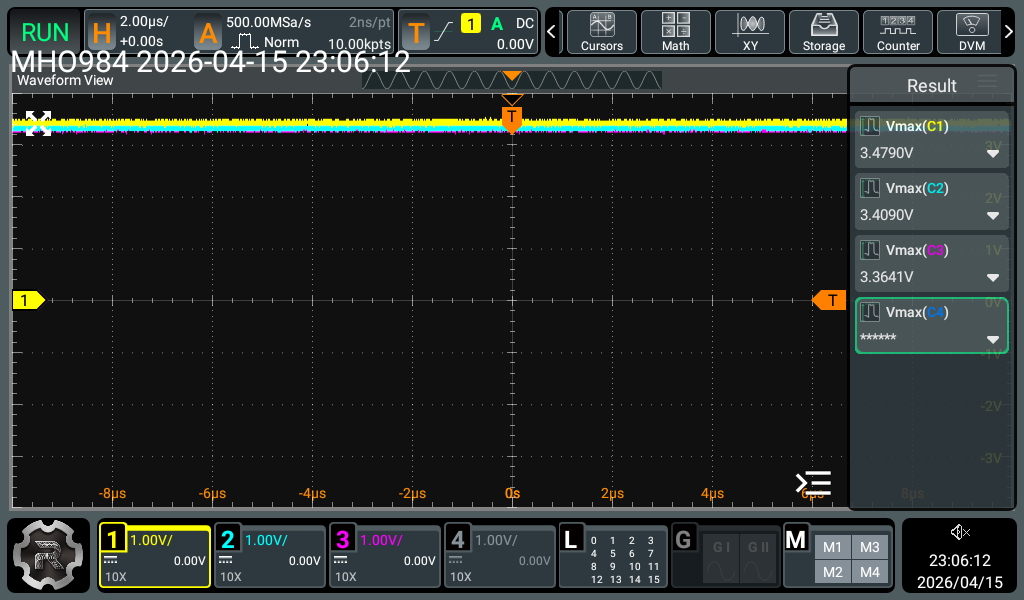
\includegraphics[width=\linewidth]{images/Chapitre 2/DCCai0.png}
    \caption{Oscilloscope measurements}
\end{subfigure}

\label{fig:dc_calibration}
\end{figure}



Based on the oscilloscope measurements, we found that
\begin{table}[H]
\centering
\caption{Measured node voltages}
\label{tab:node_voltages}
\begin{tabular}{|c|c|}
\hline
\textbf{Node} & \textbf{Measured value} \\ \hline
\texttt{VCUT} & \SI{3.409}{\volt} \\ \hline
\texttt{VTEST} & \SI{3.364}{\volt} \\ \hline
\texttt{VBNC} & \SI{3.479}{\volt} \\ \hline
\end{tabular}
\end{table}

\begin{itemize}
\item
A voltage drop of approximately \SI{45}{\milli\volt} is observed between
\texttt{VCUT} and \texttt{VTEST}. This drop is consistent with the
voltage loss across the multiplexer path, most likely caused by the
internal on-resistance of the multiplexer.

\item
An increase of approximately \SI{115}{\milli\volt} is observed between
\texttt{VTEST} and \texttt{VBNC}. This increase corresponds to the
offset measured at the \texttt{BNC} output and represents the main
effect that must be compensated during calibration.
\end{itemize}


\newpage
The following schematic provides a better explanation of the DC offset.

\begin{figure}[!htbp]
\centering
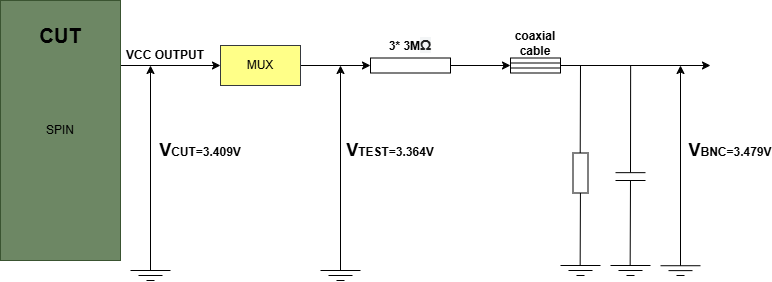
\includegraphics[width=1\textwidth]{images/Chapitre 2/SPIN_Oscilloscope_Shield-DC OFFSET.drawio.png}
\caption{DC offset schematic}
\end{figure}
To investigate this effect, the equivalent resistance formed by the three
\SI{3}{\mega\ohm} resistors was measured.

The expected equivalent resistance was approximately
\SI{9}{\mega\ohm}, while the multimeter measured about
\SI{8.8}{\mega\ohm}, corresponding to an error of approximately
\SI{2.22}{\percent}.

This result is considered acceptable since each resistor has a nominal
value of \SI{3}{\mega\ohm} with a tolerance of $\pm$\SI{5}{\percent}.


\begin{figure}[!htbp]
\centering
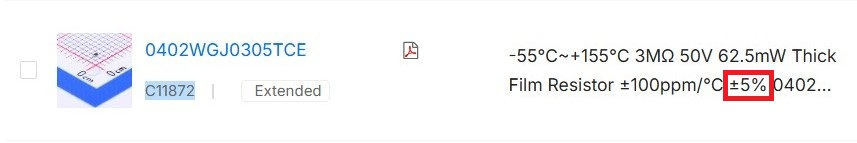
\includegraphics[width=1\textwidth]{images/Chapitre 2/Resistance.jpg}
\caption{Resistor used in the output attenuation network}
\end{figure}

With the measured resistor network, the divider is not exactly
\texttt{10x}:

\begin{align}
\frac{R_{\mathrm{scope}}}
     {R_{\mathrm{scope}} + R_{\mathrm{series}}}
  &=
    \frac{\SI{1}{\mega\ohm}}
         {\SI{1}{\mega\ohm} + \SI{8.8}{\mega\ohm}} \\
  &=
    \frac{1}{1 + 8.8} \\
  &\approx 0.102
\end{align}

Therefore, the practical correction factor is closer to
\texttt{9.8} than exactly \texttt{10}.
For more accurate measurements, the oscilloscope scaling should use this
corrected factor instead of assuming an ideal
\texttt{10x} divider. This correction is used only for
precision voltage measurements; it does not affect the routing
validation result.

\subsection{Hardware Conclusion}\label{hardware-conclusion}

The SPOC hardware has been successfully validated for the tested routing
use case.

The shield correctly routes the selected \texttt{CUT SPIN} GPIOs through
the multiplexer network to the corresponding oscilloscope channel
outputs. All four channels, all three multiplexer groups, and all routes
covered by the automatic validation sweep passed successfully.

The only remaining hardware issue is the DC offset observed at the
\texttt{BNC} output, which ranges from approximately
\SI{80}{\milli\volt} to \SI{120}{\milli\volt}. Although this offset does not affect
the functional routing validation, it should be corrected or compensated
for before using the board for accurate voltage measurements.

For the next PCB revision, two improvements are recommended. First, the
\SI{3}{\mega\ohm} divider resistors should be replaced with
lower-tolerance components. The current design uses \SI{5}{\percent}
tolerance resistors, which explains why the measured equivalent
resistance is approximately \SI{8.8}{\mega\ohm} instead of the expected
\SI{9}{\mega\ohm}. Using precision resistors would bring the equivalent
resistance closer to its nominal value and improve the accuracy of the
\texttt{10x} attenuation ratio. Second, the DC offset observed at the
\texttt{BNC} output should be compensated or corrected separately,
because it affects accurate voltage measurements independently from the
attenuation-ratio error.

\FloatBarrier


\section{Software Development and Validation}
\label{software-development-and-validation}

The second part of this chapter presents the software developed to
validate the SPOC hardware automatically. This section focuses on the
design choices, the test architecture, and the validation method used
during the project. Detailed installation and execution commands are
kept in the separate software documentation.

\subsection{Software Objective}
\label{software-objective}

The SPOC shield is designed as a generic validation board for the
\texttt{CUT SPIN}. Its purpose is to route selected signals from the
\texttt{CUT SPIN} to oscilloscope channels so that different generated
signals and communication protocols can be checked on the real hardware.
In this work, the software validation focuses on PWM signals as the
first automated test case. The host computer configures the
\texttt{CUT} firmware, commands the \texttt{MUX} firmware to select the
required route, measures the real electrical waveform with a Rigol
oscilloscope, and produces an automatic \texttt{PASS}/\texttt{FAIL}
result.

The validation framework is divided into three parts:

\begin{table}[H]
\centering
\caption{Software components used for SPOC validation}
\label{tab:software_components}
\small
\begin{tabularx}{\textwidth}{|p{3.5cm}|p{3cm}|X|}
\hline
\textbf{Component} & \textbf{Location} & \textbf{Role} \\ \hline
\texttt{Core-CUT} & CUT SPIN board & Generates PWM signals and exposes a ThingSet control interface. \\ \hline
\texttt{Core-MUX} & MUX SPIN board & Drives the multiplexer select and enable pins to route one CUT signal to one oscilloscope channel. \\ \hline
\texttt{SPOC\_Test\_Software} & Laptop & Runs the test scenarios, controls both boards, communicates with the oscilloscope, and evaluates the measurements. \\ \hline
\end{tabularx}
\normalsize
\end{table}

The framework validates the PWM behavior end to end. The laptop does not
simulate the signal; it commands the real \texttt{CUT} firmware, the
\texttt{CUT} generates an electrical waveform, the \texttt{MUX} routes
that waveform, and the oscilloscope measures it.

\begin{figure}[H]
\centering
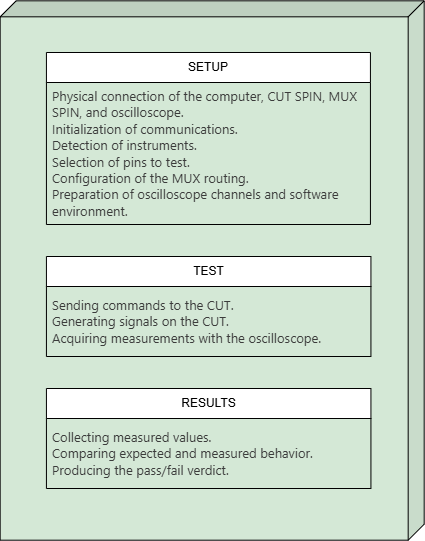
\includegraphics[width=0.56\textwidth]{images/Chapitre 2/functional_phases.png}
\caption{Functional phases of the PWM validation workflow}
\label{fig:functional_phases}
\end{figure}

\subsection{Global Software Architecture}
\label{global-software-architecture}

The software architecture follows the physical validation chain: the
laptop acts as test supervisor, sending ThingSet commands to the
\texttt{CUT} and \texttt{MUX} boards~\cite{thingset_spec}, while the
oscilloscope serves as the measurement reference, so that validation is
performed on real hardware rather than simulated PWM values.
Figure~\ref{fig:software_architecture} illustrates this architecture,
showing how the laptop communicates with both boards and how the
oscilloscope is integrated into the validation chain.

\begin{figure}[H]
\centering
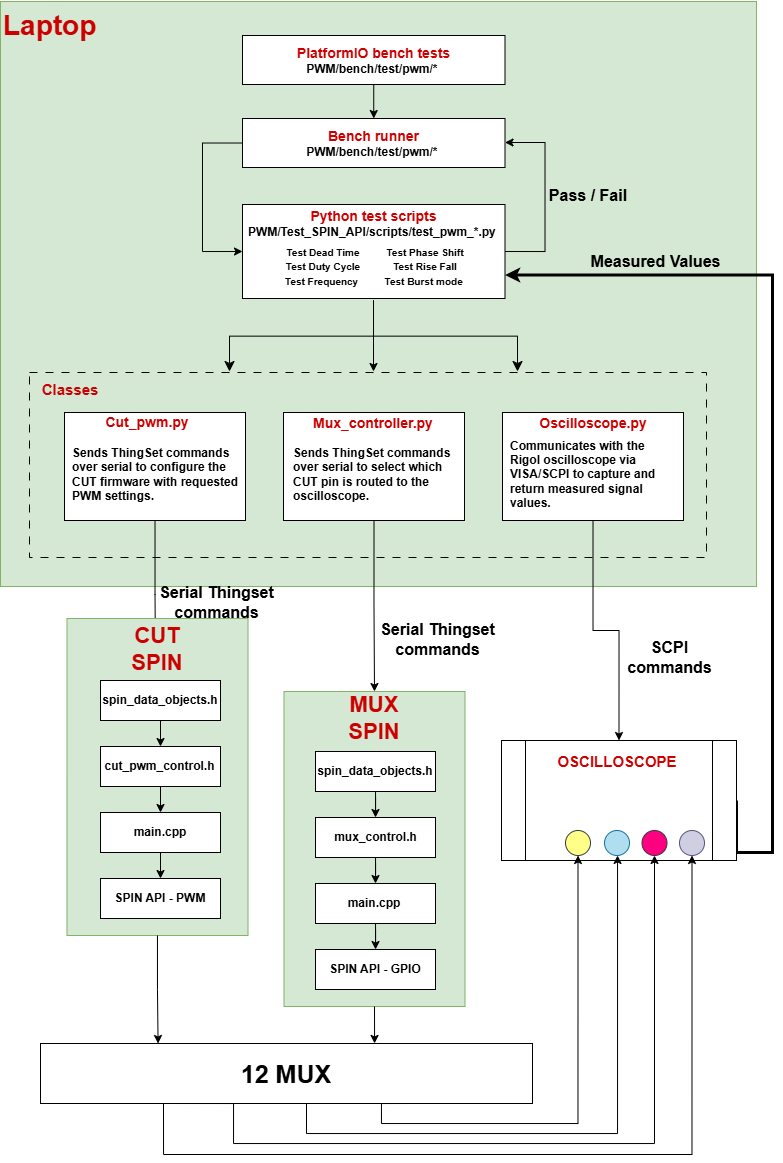
\includegraphics[width=0.71\textwidth]{images/Chapitre 2/Software_Architecture.png}
\caption{Software architecture}
\label{fig:software_architecture}
\end{figure}

\subsection{Firmware Architecture: \texttt{Core-CUT}}
\label{firmware-architecture-core-cut}

\texttt{Core-CUT} is the firmware running on the SPIN board under test.
It exposes a compact ThingSet API and translates commands sent by the
laptop into real PWM configurations applied through the OwnTech
\texttt{SpinAPI} and HRTIM layer, making it the source of the electrical
signal measured during validation.

The firmware stores the requested PWM configuration in a shared state
and applies it only when the host triggers the apply command, avoiding
partial configurations being propagated to the PWM outputs while
several parameters are being updated.

\begin{table}[H]
\centering
\caption{Main responsibilities of the \texttt{Core-CUT} firmware}
\label{tab:core_cut_responsibilities}
\small
\begin{tabularx}{\textwidth}{|p{4.5cm}|X|}
\hline
\textbf{Element} & \textbf{Responsibility} \\ \hline
\texttt{src/main.cpp} & Initializes the firmware, stores the PWM state, applies the requested configuration, and starts or stops the selected outputs. \\ \hline
\texttt{cut\_pwm\_control.h} & Defines the shared PWM state and the \texttt{cut\_pwm\_apply()} function used by the ThingSet callback. \\ \hline
\texttt{spin\_data\_objects.h} & Exposes the \texttt{/Cut/PwmOut} ThingSet objects used by the laptop to configure the CUT. \\ \hline
\texttt{SpinAPI / HRTIM} & Generates the physical PWM waveforms on the selected SPIN pins. \\ \hline
\end{tabularx}
\normalsize
\end{table}

The laptop first writes the desired values under \texttt{/Cut/PwmOut},
including frequency, duty cycle, phase shift, dead time, modulation
mode, switch convention, and output-enable state. When the host writes
the \texttt{xApply} object, the ThingSet callback calls
\texttt{cut\_pwm\_apply()}: the previous PWM state is cleared, the
selected timing units are configured, and the enabled outputs are
started, making the resulting waveform available on the physical
\texttt{CUT SPIN} pins.

\begin{table}[H]
\centering
\caption{Main \texttt{Core-CUT} ThingSet objects used by the tests}
\label{tab:core_cut_thingset_objects}
\small
\begin{tabularx}{\textwidth}{|p{4.5cm}|X|}
\hline
\textbf{Object group} & \textbf{Purpose} \\ \hline
\texttt{wFreq\_Hz}, \texttt{wMinFreq\_Hz}, \texttt{wMod}, \texttt{wEnable}, \texttt{xApply} & Global PWM configuration and apply trigger. \\ \hline
\texttt{wA1} to \texttt{wF2} & Enable flags for the PWM timing-unit outputs. \\ \hline
\texttt{wADuty} to \texttt{wFDuty} & Duty-cycle commands for each PWM unit. \\ \hline
\texttt{wAPhase\_deg} to \texttt{wFPhase\_deg} & Phase-shift commands used by two-output tests. \\ \hline
\texttt{wADeadRise}/\texttt{wADeadFall} to \texttt{wFDeadRise}/\texttt{wFDeadFall} & Rising and falling dead-time configuration. \\ \hline
\texttt{wAMod} to \texttt{wFMod} & Modulation-mode selection, including left-aligned and up-down PWM. \\ \hline
\texttt{wASwitchConv} to \texttt{wFSwitchConv} & PWMx1/PWMx2 switch-convention selection. \\ \hline
\texttt{rStatus}, \texttt{rAPeriod} to \texttt{rFPeriod} & Readback objects used for diagnostics and resolution checks. \\ \hline
\end{tabularx}
\normalsize
\end{table}

In the host mapping, the tested PWM outputs cover the SPIN pins
\texttt{PA8}, \texttt{PA9}, \texttt{PA10}, \texttt{PB12},
\texttt{PB13}, \texttt{PB14}, \texttt{PB15}, \texttt{PC6},
\texttt{PC7}, \texttt{PC8}, and \texttt{PC9}, linking each pin to its
corresponding PWM unit and timing unit and allowing the same test
scripts to run on one pin or on a complete pin matrix.


\subsection{Firmware Architecture: \texttt{Core-MUX}}
\label{firmware-architecture-core-mux}

\texttt{Core-MUX} is the firmware running on the second SPIN board. Its
role is to control the external analog multiplexers of the SPOC shield.
For each oscilloscope channel, the firmware drives four select lines
\texttt{S0..S3} and the enable lines of the three mux groups. In this
way, a GPIO signal coming from the \texttt{CUT SPIN} can be connected to
one selected oscilloscope input path.

The MUX firmware is simpler than the CUT firmware: it does
not generate signals, it only applies a routing state. The host selects a
mux input index and an oscilloscope channel, then the firmware disables
the previous route, updates the select pins, and enables the selected
mux output.

\begin{table}[H]
\centering
\caption{Main responsibilities of the \texttt{Core-MUX} firmware}
\label{tab:core_mux_responsibilities}
\small
\begin{tabularx}{\textwidth}{|p{4.5cm}|X|}
\hline
\textbf{Element} & \textbf{Responsibility} \\ \hline
\texttt{src/main.cpp} & Defines the GPIO mapping, configures the mux control pins, stores route states, and applies the requested routes. \\ \hline
\texttt{mux\_control.h} & Defines the route-state contract shared between the hardware layer and the ThingSet layer. \\ \hline
\texttt{spin\_data\_objects.h} & Exposes the \texttt{/Mux/MuxX/ChY} ThingSet objects used by the host software. \\ \hline
\texttt{SpinAPI GPIO} & Drives the select and enable pins connected to the analog multiplexers. \\ \hline
\end{tabularx}
\normalsize
\end{table}

Each oscilloscope channel has its own routing group. The four select
pins encode the input index, while the enable pins select which mux
group is active for that channel.

\begin{table}[H]
\centering
\caption{\texttt{Core-MUX} routing groups}
\label{tab:core_mux_routing_groups}
\small
\begin{tabularx}{\textwidth}{|X|X|X|}
\hline
\textbf{Routing group} & \textbf{Select pins} & \textbf{Enable pins} \\ \hline
\texttt{Ch1} & \texttt{PA0}, \texttt{PA1}, \texttt{PA2}, \texttt{PA3} & \texttt{PC0}, \texttt{PC1}, \texttt{PC2} \\ \hline
\texttt{Ch2} & \texttt{PA4}, \texttt{PA5}, \texttt{PA6}, \texttt{PA7} & \texttt{PC3}, \texttt{PC4}, \texttt{PC5} \\ \hline
\texttt{Ch3} & \texttt{PB0}, \texttt{PB1}, \texttt{PB2}, \texttt{PB3} & \texttt{PC6}, \texttt{PC7}, \texttt{PC8} \\ \hline
\texttt{Ch4} & \texttt{PB4}, \texttt{PB5}, \texttt{PB6}, \texttt{PB7} & \texttt{PC9}, \texttt{PC10}, \texttt{PC11} \\ \hline
\end{tabularx}
\normalsize
\end{table}

The routing command follows the same pattern as the CUT configuration.
The laptop writes \texttt{/Mux/MuxX/ChY/wChannel} and
\texttt{/Mux/MuxX/ChY/wEnable}, then executes
\texttt{/Mux/MuxX/ChY/xApply}. The firmware updates the selected route,
masks the requested channel to the four-bit mux input range, disables
the previous route for the selected output path, applies the select
lines, and enables the correct mux group. 


\subsection{Host Software Architecture: \texttt{SPOC\_Test\_Software}}
\label{host-software-architecture-spoc-test-software}

\texttt{SPOC\_Test\_Software} is the Python layer executed on the
laptop, linking the embedded firmware and the measurement instrument
into one automated validation loop, launched either through direct
Python scripts during debugging or through PlatformIO bench suites
during repeated validation.

Its main role is orchestration: it opens serial connections to the
\texttt{CUT} and \texttt{MUX} boards, enters ThingSet mode, sends PWM
and routing commands, configures the oscilloscope through VISA/SCPI
using PyVISA~\cite{rigol_mho900_programming,pyvisa_docs}, reads the
measured values, and compares them with the expected result.

\subsubsection{Main Software Classes}
\label{main-software-classes}

The host software is organized around a small set of Python classes,
each isolating one communication responsibility so that validation
scripts do not directly manage serial commands, mux routing, or
oscilloscope SCPI instructions.

\begin{table}[H]
\centering
\caption{Main host-side controller classes}
\label{tab:host_controller_classes}
\small
\begin{tabularx}{\textwidth}{|p{4.5cm}|X|}
\hline
\textbf{Class} & \textbf{Role} \\ \hline
\texttt{CutPwmController} & Maps real pin names such as \texttt{PA8} to PWM units and writes the corresponding \texttt{/Cut/PwmOut} ThingSet objects. \\ \hline
\texttt{MuxController} & Maps a CUT pin to its mux number and input index, then routes it to the selected oscilloscope channel. \\ \hline
\texttt{OscilloscopeClient} / \texttt{Oscilloscope} & Manages the VISA/SCPI session, configures channels and triggers, and reads timing or voltage measurements. \\ \hline
\texttt{ThingSetShell} & Provides the shared serial layer used to read, write, and execute ThingSet objects on both embedded boards. \\ \hline
\end{tabularx}
\normalsize
\end{table}

\texttt{CutPwmController} converts test parameters such as pin name,
frequency, duty cycle, phase shift, or dead time into the ThingSet
objects exposed by \texttt{Core-CUT}. \texttt{MuxController} identifies
which mux group and input index correspond to a selected \texttt{CUT}
pin and routes it to the requested oscilloscope channel.
\texttt{Oscilloscope} configures the Rigol oscilloscope and reads the
required values, such as frequency, duty cycle, rise/fall time, delay,
and pulse width. \texttt{ThingSetShell} is the shared low-level layer
providing the read, write, and execute operations used by both
controllers.

The host execution flow starts from a direct script or a PlatformIO
bench command: PlatformIO loads a custom runner, reads the selected
\texttt{bench\_config.json}, converts the environment variables into
script arguments, and launches the Python test, which connects to the
hardware, applies the CUT configuration and MUX route, configures the
oscilloscope, reads the measurements, and exits with a status code
representing \texttt{PASS}, \texttt{FAIL}, or configuration error.

This architecture centralizes hardware communication inside controller
classes, so each validation script can focus on the test criterion
itself: signal, route, measurement, and tolerance.


\subsection{Automated Validation Procedure}
\label{automated-validation-procedure}

Each automated test follows the same general sequence. The host first
configures the PWM output on the CUT board, then asks the MUX board to
route the selected pin to an oscilloscope channel. After the signal is
stable, the oscilloscope is configured and the required measurements are
read. Finally, the script compares the measured values with the expected
values and returns a \texttt{PASS} or \texttt{FAIL} result.

\begin{figure}[H]
\centering
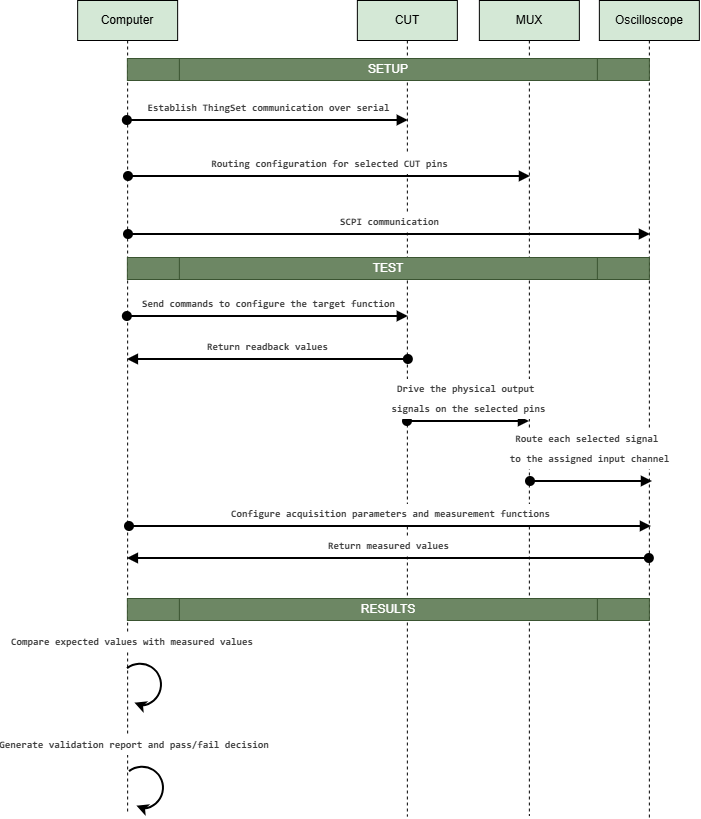
\includegraphics[width=0.92\textwidth]{images/Chapitre 2/sequence_diagram.png}
\caption{Host, CUT, MUX, and oscilloscope validation sequence}
\label{fig:software_sequence_diagram}
\end{figure}



\subsection{Implemented Validation Tests}
\label{implemented-validation-tests}

Nine PWM validation tests were implemented. They cover both basic PWM
generation and more advanced timing features such as complementary
outputs, phase shift, and burst mode.

\begin{table}[H]
\centering
\caption{Implemented PWM validation tests}
\label{tab:implemented_pwm_tests}
\small
\begin{tabularx}{\textwidth}{|p{3.5cm}|X|}
\hline
\textbf{Test} & \textbf{Validation purpose and pass criterion} \\ \hline
Duty cycle & Checks that the measured duty cycle matches the value requested by the host script within the configured tolerance. \\ \hline
Frequency & Confirms that the \texttt{CUT} generates the requested PWM carrier frequency and that the oscilloscope measurement stays within percentage tolerance. \\ \hline
Rise/fall time & Measures the electrical transition speed of the PWM output and verifies that both rise and fall times remain below the configured limits. \\ \hline
Dead time & Measures the delay between complementary PWM outputs and checks that rising and falling dead times match the configured values within tolerance. \\ \hline
Phase shift & Measures the delay between two PWM outputs, converts it to degrees, and compares it with the requested phase shift. \\ \hline
Burst mode & Validates the reduced burst-mode interface by checking that burst period and active/off timing agree with the configured cycle counts. \\ \hline
Modulation modes & Verifies that frequency and duty cycle remain valid in both left-aligned and up-down PWM modes. \\ \hline
Switch convention & Checks that PWMx1/PWMx2 output behavior follows the selected convention, including complementary behavior when expected. \\ \hline
Resolution & Verifies the timer resolution selected during variable-frequency initialization using the generated frequency and, when available, firmware readback. \\ \hline
\end{tabularx}
\normalsize
\end{table}

\subsection{Software Validation Results}
\label{software-validation-results}

The software validation confirmed that the host can control the complete
test chain: PWM generation on the CUT board, signal routing through the
MUX board, oscilloscope configuration, measurement acquisition, and
automatic decision reporting. The same scripts can be used for a single
pin during debugging or for broader pin and pair matrices during
regression testing.

The main validation result is that the framework provides repeatable
end-to-end measurements instead of manual oscilloscope checks. This is
important for the SPOC project because it allows the hardware routing and
the PWM behavior of the CUT to be tested together under the same
procedure.

\subsection{HRTIM Burst Mode Issue and Correction}
\label{hrtim-burst-mode-issue-and-correction}

During the PWM burst-mode validation, the automated test bench revealed
an off-by-one behavior in the STM32 HRTIM burst-mode configuration used
by the OwnTech SPIN firmware. This issue was not caused by the SPOC
shield routing hardware. It was observed on the real PWM waveform while
testing the \texttt{CUT SPIN} through the complete validation chain.

The issue appeared when configuring the HRTIM burst mode with
\texttt{HRTIM\_BMCMP} and \texttt{HRTIM\_BMPER}. The HRTIM
burst-mode behavior was analyzed using the STM32G4 reference manual
and the HRTIM application note~\cite{st_rm0440,st_an4539}. The tested
firmware configuration was equivalent to:

\begin{small}
\begin{verbatim}
LL_HRTIM_BM_SetCompare(HRTIM1, 7);
LL_HRTIM_BM_SetPeriod(HRTIM1, 10);
\end{verbatim}
\end{small}

The expected burst pattern was \texttt{7} inactive cycles,
\texttt{3} active cycles, and \texttt{10} total cycles. However, the
oscilloscope showed \texttt{8} inactive cycles, \texttt{3} active
cycles, and \texttt{11} total cycles. The measured time between two
burst patterns was \SI{8.75}{\milli\second} instead of the expected
\SI{7.5}{\milli\second}.

\begin{figure}[H]
\centering
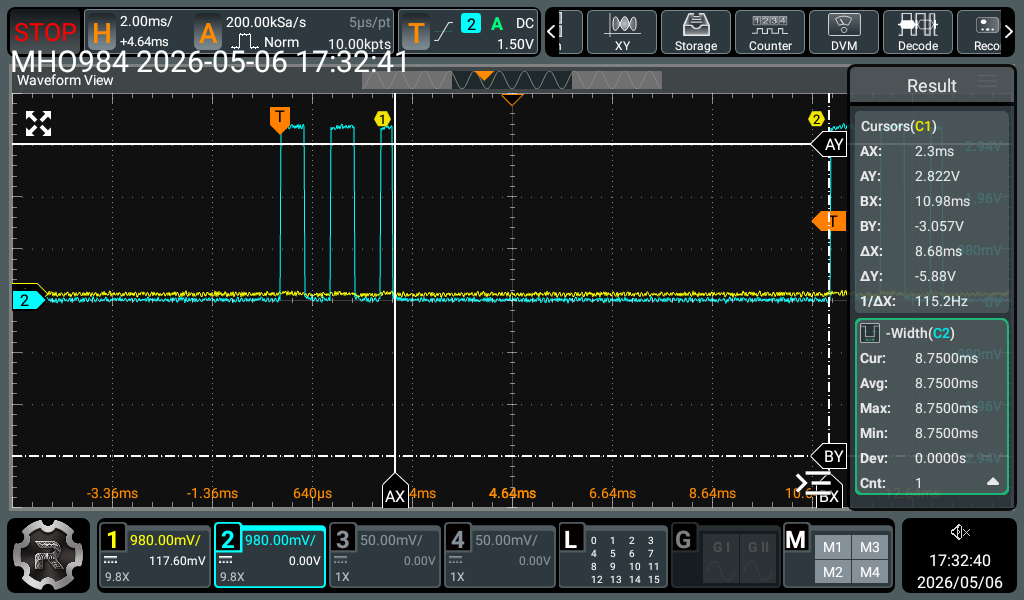
\includegraphics[width=0.70\textwidth]{images/Chapitre 2/burst.png}
\caption{Observed burst-mode timing error on the oscilloscope}
\label{fig:burst_mode_timing_error}
\end{figure}

The difference between the expected and measured burst periods is
\SI{1.25}{\milli\second}. The main part of this error corresponds to the
off-by-one cycle added by the HRTIM burst counter. A smaller remaining
time error, approximately \SI{0.25}{\milli\second}, was also observed
and is related to the final PWM pulse being truncated at the end of the
burst sequence. The off-by-one behavior was therefore the first issue to
correct because it directly changed the number of inactive and total
cycles programmed by the software.

The root cause is that the HRTIM burst-mode counter is zero-based and
inclusive. In other words, the hardware counts from \texttt{0} to the
programmed register value. Therefore, the real number of cycles is one
more than the value written to the register:

\begin{align}
\text{real inactive cycles} &= \texttt{HRTIM\_BMCMP} + 1 \\
\text{real total cycles} &= \texttt{HRTIM\_BMPER} + 1
\end{align}

\begin{figure}[H]
\centering
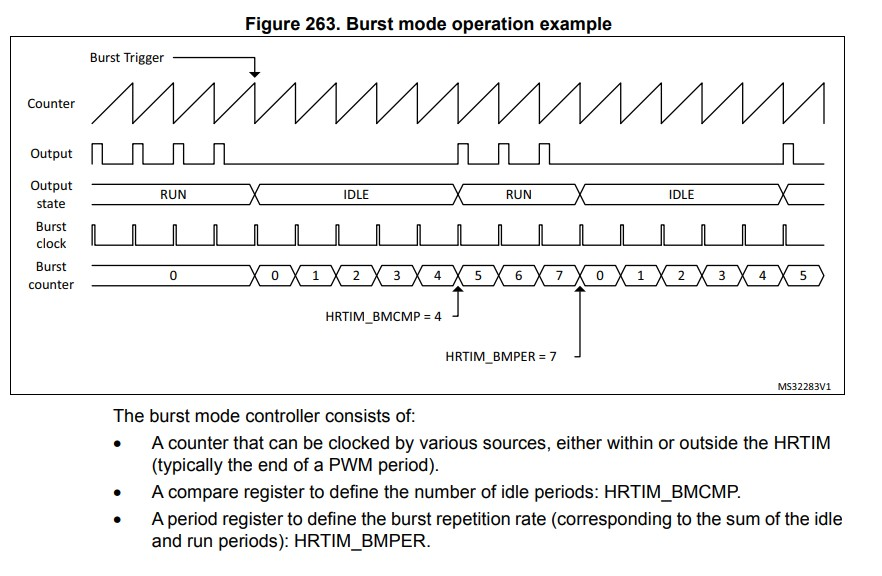
\includegraphics[width=0.90\textwidth]{images/Chapitre 2/burst mode datasheet.jpg}
\caption{STM32 HRTIM burst-mode counter behavior from the reference manual}
\label{fig:burst_mode_datasheet}
\end{figure}



The correction consists of converting the user-facing cycle counts into
hardware register values before programming the HRTIM registers. The
compare and period values are decremented by one:


\begin{small}
\begin{verbatim}
Before correction:

LL_HRTIM_BM_SetCompare(HRTIM1, bm_cmp);
LL_HRTIM_BM_SetPeriod(HRTIM1, bm_per);
\end{verbatim}
\end{small}

\begin{small}
\begin{verbatim}
After correction:

LL_HRTIM_BM_SetCompare(HRTIM1, bm_cmp - 1);
LL_HRTIM_BM_SetPeriod(HRTIM1, bm_per - 1);
\end{verbatim}
\end{small}



After this correction, a command requesting \texttt{7} inactive cycles
and \texttt{10} total cycles produces the expected burst pattern. The
test therefore confirmed that the SPOC validation software reached its
objective: it automated PWM validation and also made it possible to
detect, analyze, and correct a real firmware issue in the SPIN PWM
stack.

\subsection{Software Conclusion}
\label{software-conclusion}

The developed software completes the SPOC validation platform by adding
automated control and measurement around the hardware shield. The
\texttt{Core-CUT} firmware generates configurable PWM signals, the
\texttt{Core-MUX} firmware selects the measurement path, and the Python
host software coordinates the full validation loop with the oscilloscope.

This software structure makes the validation process faster, more
repeatable, and less dependent on manual oscilloscope configuration. It
also provides a foundation for future tests beyond PWM, since the same
CUT, MUX, and oscilloscope control architecture can be extended to other
signals and communication protocols. In addition, the
burst-mode investigation showed that the validation framework is able to
identify implementation issues in the tested SPIN firmware.

This confirms the importance of a dedicated validation board before
releasing products to the market. Some defects may not appear during
normal use, so an automatic test platform able to exercise the signals
and verify the board behavior systematically is necessary to increase
confidence in the final product.


\FloatBarrier

